%=======================+=========================
%================  Introduction  ================
%=================================================
\section[The \gx{} experiment]{\label{sec:gluexexperiment} The \gx{} experiment}
The search for Quantum ChromoDynamics (QCD) exotics uses data from a wide range of experiments and production mechanisms. Historically, the searches have looked for the gluonic excitations of mesons, searching for states of pure glue, glueballs, and hybrid mesons where the gluonic field binding the quark-anti-quark pair has been excited. Most experiments searching for glueballs looked for scalers~\cite{Crede:2008vw}, where the searches relied on over-population of nonets, as well as unusual meson decay patterns. In the search for hybrid mesons~\cite{Meyer:2010ku,Meyer:2015eta}, efforts have focused on particles with exotic quantum numbers, that is systems beyond simple quark-anti-quark configurations. Good evidence exists for an isospin $1$ state, the $\pi_{1}(1600)$. Looking collectively at past studies, data from high-statistics photoproduction experiments in the energy range above $6$~GeV is lacking. 

\begin{figure}[hbt]\centering
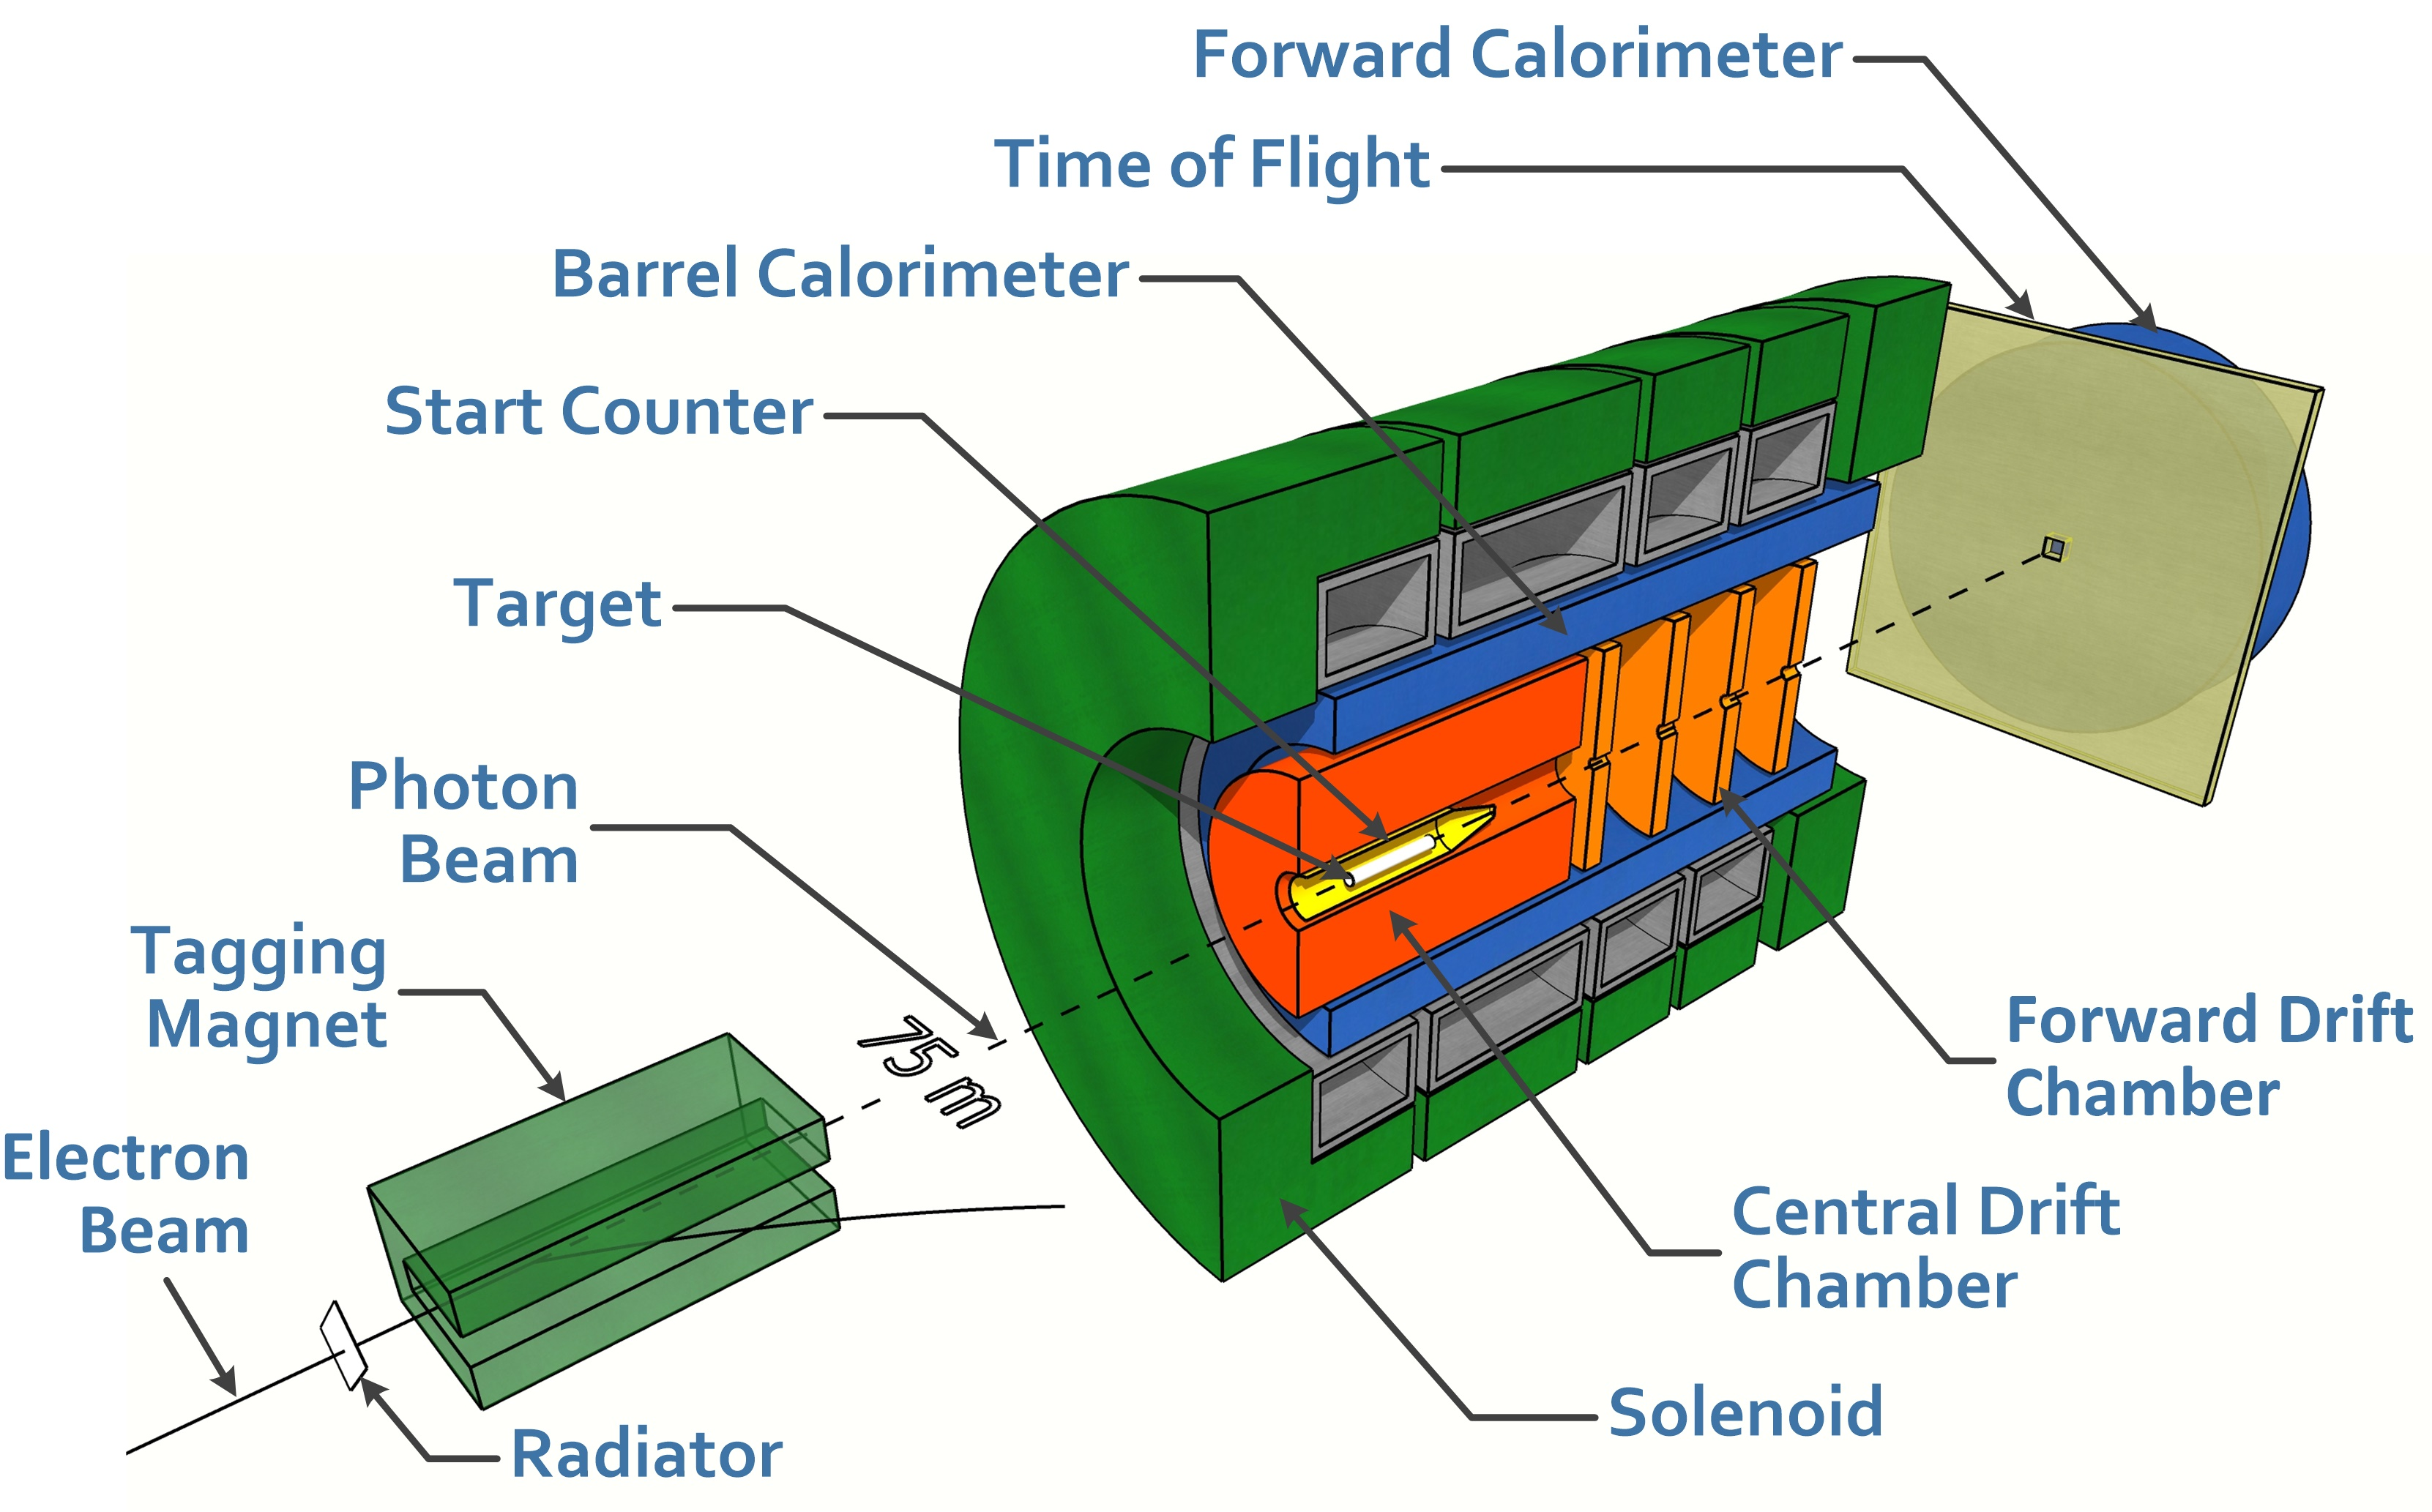
\includegraphics[width=0.75\textwidth]{figures/GlueX-graphic.jpg}
\caption[]{\label{fig:gluex_cut-away}(Color online)A cut-away drawing of the \GX{} detector in Hall D, not to scale.}
\end{figure}
The \emph{Glu}onic \emph{Ex}citation (\gx{}) experiment at the 
US Department of Energy's Thomas Jefferson National Accelerator Facility (JLab)\footnote{Thomas Jefferson National Accelerator Facility, 12000 Jefferson Ave., Newport News, VA 23606, https://www.jlab.org.} has been built to both search for and map out the spectrum of exotic hybrid mesons using a 9-GeV linearly-polarized photon beam incident on a proton target\cite{gluex-ref}. The \gx{} detector and beamline are shown schematically in Figure~\ref{fig:gluex_cut-away}. The detector is nearly hermetic for both charged particles and photons arising from reactions in the cryogenic target at the center of the detector, allowing for reconstruction of exclusive final states. A 2-T solenoidal magnet surrounds the drift chambers used for charged-particle tracking. Two electromagnetic calorimeters cover the central and forward regions, and a scintillation detector downstream provides particle-identification capability through time-of-flight measurements. 


\subsection[The Hall-D complex]{The Hall-D complex \label{sec:gluexexperiment:complex}}
The \gx{} experiment is housed in the Hall-D complex at JLab (see Fig.\ref{fig:CEBAF-graphic}). This new facility starts with an extracted electron beam at the north end of the Continuous Electron Beam Accelerator Facility (CEBAF) \cite{Leemann:2001dg}. The electron beam is delivered to the Tagger Hall, where the maximum energy is 12~GeV, due to an extra one-half pass of acceleration relative to three other experimental halls (A, B and C).  Here, linearly-polarized photons are produced through coherent bremsstrahlung off a 50~$\mu$m thick diamond crystal radiator.
The scattered electrons pass through a tagger magnet and are bent into tagging detectors. A high-resolution scintillating-fiber tagging array covers the 8 to 9~GeV energy range, and a tagger hodoscope covers photon energies both from 9~GeV to the endpoint, and from 8~GeV to 3~GeV. Electrons not interacting in the diamond are directed into a 60 kW electron beam dump. The tagged photons travel to the Hall-D experimental hall. The distance from the radiator to the primary collimator is 75~m. The collimator, with a diamter of 5~mm diameter, removes off-axis incoherent photons. The front face of the collimator is instrumented with an active collimator to aid in beam tuning.  The beamline and tagging system are described below in Section\,\ref{sec:beamline}.

Downstream of the primary collimator is a thin beryllium radiator used by both the Triplet Polarimeter, which measures the linear polarization of the photons, and a Pair Spectrometer, which is used to measure the flux of the photons. More information on the production, tagging and monitoring of the photon beam can be found in Section~\ref{sec:beamline}. 
The photon beam continues through to a liquid hydrogen target at the heart of the \gx{} detector, and then to the end of the experimental hall where it enters the photon beam dump.

\begin{figure}[tbp]\centering
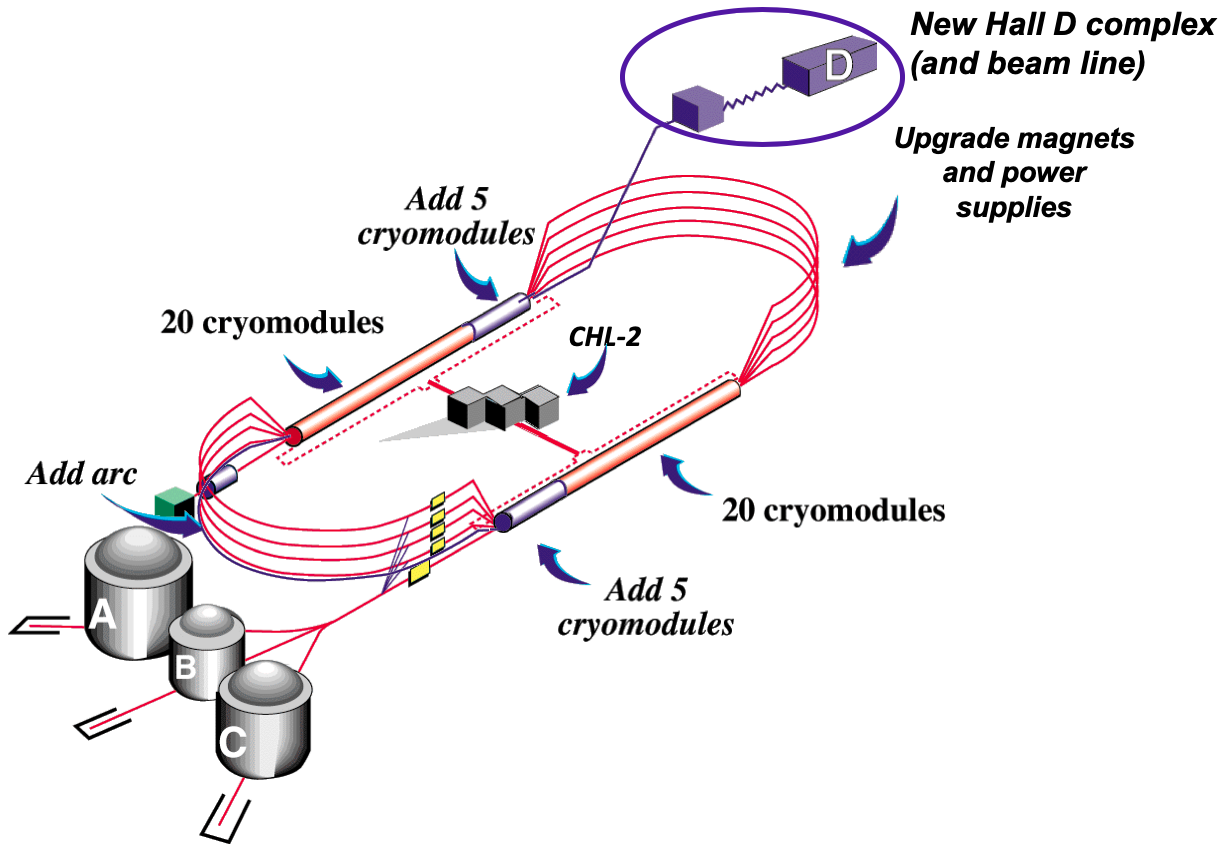
\includegraphics[width=0.75\textwidth]{figures/CEBAF-graphic.png}
\caption[]{\label{fig:CEBAF-graphic}(Color online) Schematic of the CEBAF accelerator showing the additions made during the 12-GeV project. The Hall D complex is located at the north-east end.}
\end{figure}

The layout of the \gx{} detector is shown in Fig.~\ref{fig:layout_spectrometer}. The spectrometer is based on a 4-m-long solenoidal magnet that is operated at a maximum field of 2~T, see Section~\ref{sec:solenoid}. The liquid-hydrogen target is located 65~cm inside the upstream bore of the magnet. The target consists of a 2-cm-diameter, 30-cm-long volume of hydrogen, as described in Section~\ref{sec:target}. Surrounding the target is the Start Counter, which consists of 30 thin scintillator paddles that bend to a nose on the down-stream end of the hydrogen target. The Start Counter is the primary detector that registers the time coincidence of the radio-frequency (RF) bunch containing the incident electron and the tagged photon producing the interaction. More information on the scintillator detector can be found in Section~\ref{sec:scintillators}. 

% ======================================================================================

\begin{figure*}[tbp]
\centering
  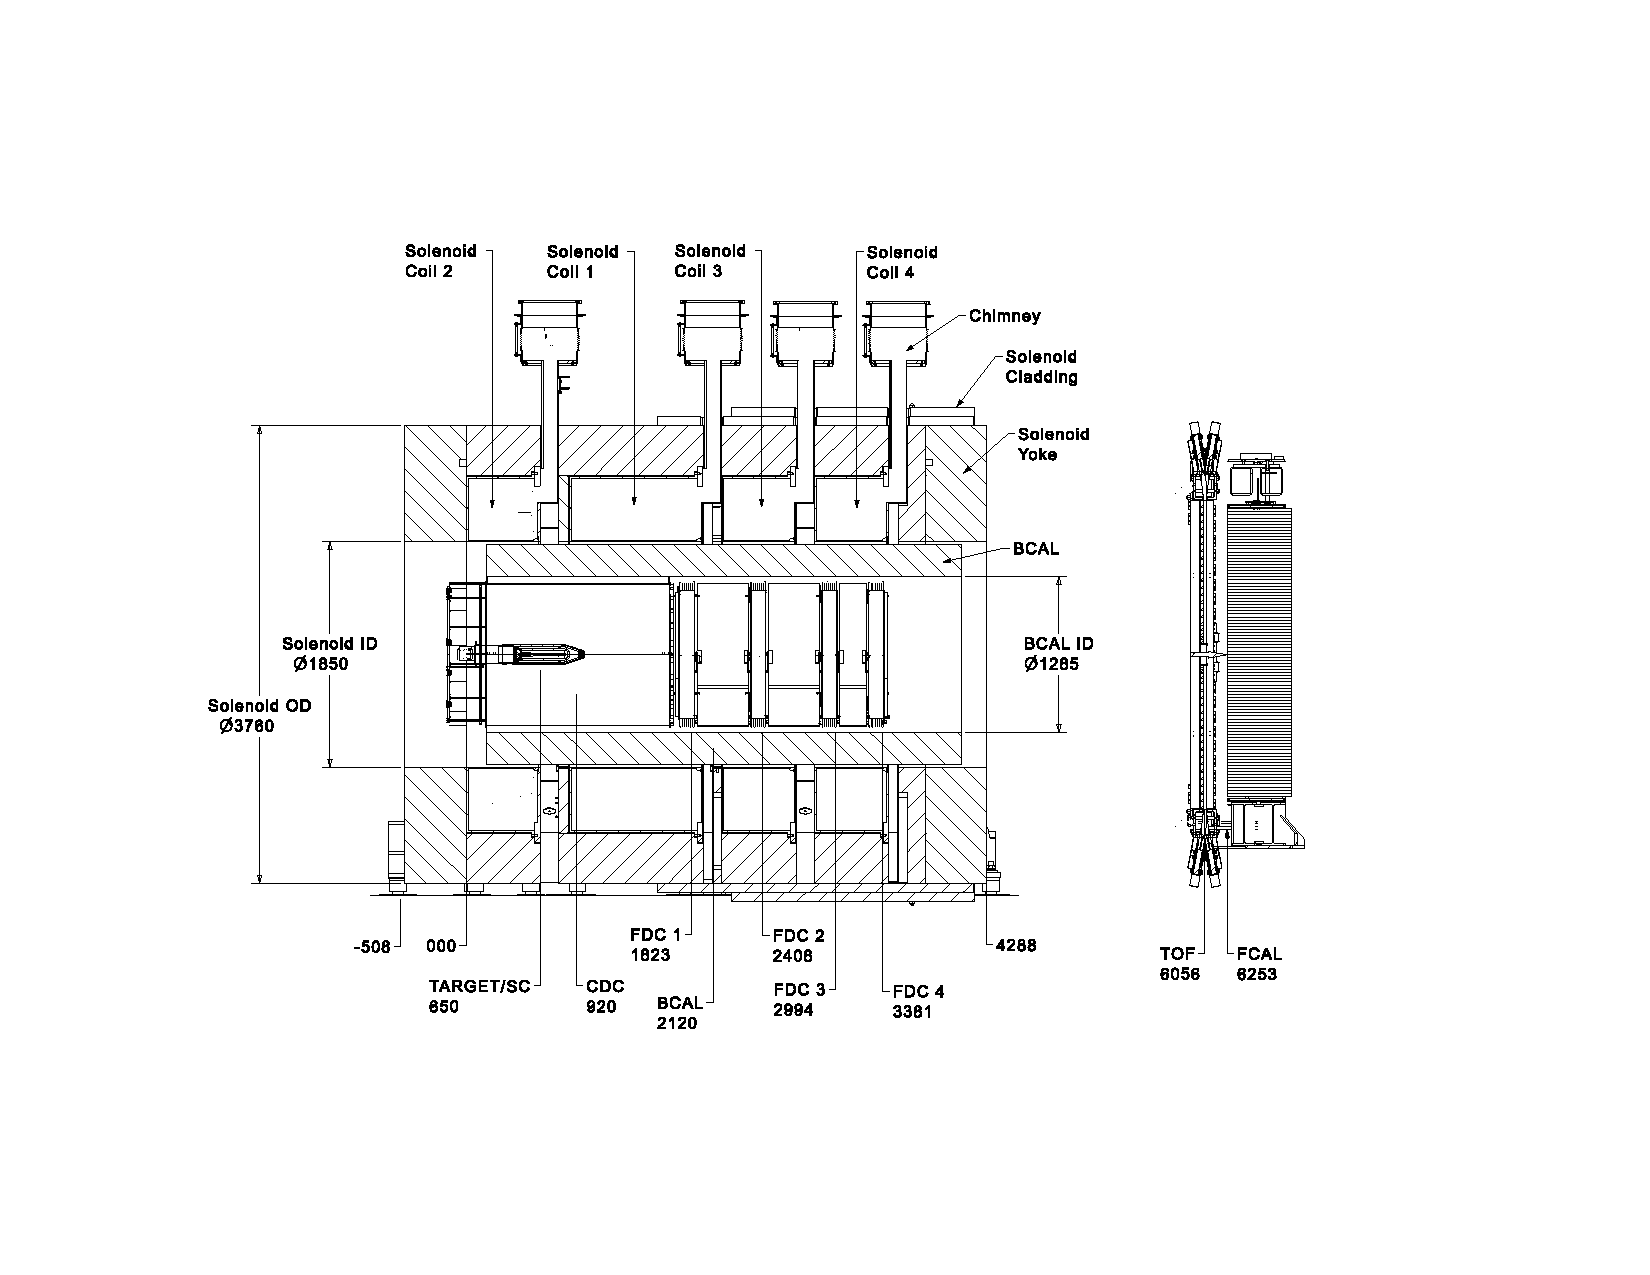
\includegraphics[angle=0,viewport=95 115 628 500,clip,width=1.0\linewidth]{figures/gluex_spectrometer_drawing_01_bw}%
  \caption[layout]{GlueX spectrometer layout. Dimensions are given in mm. The
    numbers show the Z-coordinates of the detectors' centers, or of
    the front face of the calorimeter modules in case of the FCAL.
    Glossary: 
              SC  - Start Counter (Section \ref{sec:st}), 
              CDC - Central Drift Chamber (Section \ref{sec:cdc}), 
              FDC - Forward Drift Chamber (Section \ref{sec:fdc}),
              BCAL - Barrel Calorimeter (Section \ref{sec:bcal}), 
              TOF -  Time-of-Flight hodoscope (Section \ref{sec:tof}), 
              FCAL - Forward Calorimeter (Section \ref{sec:fcal}).
%
%    \begin{tabular}{lll}
%       Name  & Detector & Section \\ \hline
%              SC  & Start Counter & \ref{sec:st} \\ 
%              CDC & Central Drift Chamber  & \ref{sec:cdc} \\ 
%              FDC & Forward Drift Chamber  & \ref{sec:fdc} \\ 
%              BCAL & Barrel Calorimeter    & \ref{sec:bcal} \\ 
%              TOF &  Time-of-Flight hodoscope & \ref{sec:tof} \\ 
%              FCAL & Forward Calorimeter    & \ref{sec:fcal} \\ 
%    \end{tabular}
    \label{fig:layout_spectrometer}
  }
\end{figure*}

% ======================================================================================


%\begin{figure}[htbp]\centering
%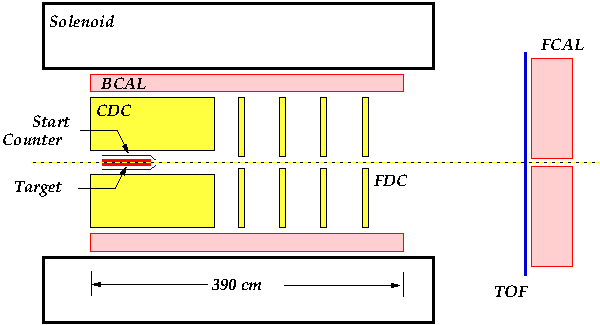
\includegraphics[width=0.7\textwidth]{figures/GlueX_Sketch.pdf}  
%\caption{\label{fig:gluexsketch} (Color online)         
%Sketch of GlueX detector.  The main systems of the detector are the Start %Counter \cite{Pooser:2019rhu}, the Central Drift Chamber (CDC) %\cite{VanHaarlem:2010yq} the Forward Drift Chamber (FDC) \cite{Pentchev2017281}, %a scintillator-based Time of Flight (TOF) wall and a lead-glass Forward %Calorimeter (FCAL) \cite{MORIYA201360}. The Barrel Calorimeter (BCAL) is %sandwiched between the drift chambers and the inner radius of the solenoid.}   
%\end{figure}

Starting at a radius of 10~cm from the beam line is the Central Drift Chamber, a cylindrical straw-tube detector. The active volume of the chamber extends from 48~cm upstream to 102~cm downstream of the target center, and from 10~cm to 56~cm in radius. The Central Drift Chamber consists of 28 layers of straw tubes in axial and two stereo orientations. Downstream of the central tracker is the Forward Drift Chamber, which consists of four packages, each containing 6 planar layers in alternating $u$-$y$-$v$ orientations. Both cathodes and anodes in the Forward Drift Chamber are read out, providing three-dimensional space point measurements. More details on the tracking system are provided in Sections~\ref{sec:tracking} and \ref{sec:trackingperformance}. 

Downstream of the magnet is the Time-of-Flight wall. This system consists of two layers of scintillator paddles in a crossed pattern, and, in conjunction with the Start Counter, is used to measure the flight time of charged particles. More information on the time-of-flight system is provided in Section~\ref{sec:scintillators}. 
Photons arising from interactions within in the \gx{} target are detected by two calorimeter systems. The Barrel Calorimeter, located inside the solenoid, consists of layers of scintillating fibers alternating with lead sheets. The Forward Calorimeter is downstream of the Time-of-Flight wall, and consists of $2800$ lead-glass blocks. More information on the the calorimeters can be found in Section~\ref{sec:calorimeters}.

\subsection[Experimental requirements]{Experimental requirements \label{sec:intro:requirements}}
The physics goals of the GlueX experiment require the reconstruction of exclusive final states. Thus, the \gx{} detector must be able to reconstruct both charged particles ($\pi^{\pm}$, $K^{\pm}$ and $p/\bar{p}$) and particles decaying into photons ($\pi^{\circ}$, $\eta$, $\omega$ and $\eta^{\prime}$). For this capability, the charged particles and photons must be reconstructed with good momentum and energy resolution. The experiment must also be able to reconstruct the energy of the incident photon (8 to 9~GeV) with high accuracy ($0.1$\%) and have knowledge of the linear polarization (maximum $\sim$40\%) of the photon beam to an absolute precision of 1\%. Finally, many interesting final states involve more than five particles. Thus, the \gx{} detector must also be nearly hermetic for both charged particles and photons, with an acceptance that is reasonably uniform, well understood, and accurately modeled in simulation.

In practice, the typical momentum resolution for charged particles is $1$--$3\%$, while the resolution is 8-9\% for very-forward high-momentum particles.  For most charged particles, the tracking system has nearly hermetic acceptance for polar angles from $1^\circ-2^{\circ}$ to $150^{\circ}$. However, protons with momenta below about 250~MeV/c are absorbed in the hydrogen target and not detected. A further challenge is the reconstruction of tracks from charged pions with momenta under 200~MeV/c due to spiraling trajectories in the magnetic field.
The measurement of energy loss ($dE/dx$) in the Central Drift Chamber enables the separation of pions and protons up to about 800~MeV/c, while time-of-flight determination allows separation of forward-going pions and kaons up to about 2~GeV/c.

For photons produced from the decays of reaction products, the typical energy resolution is 5 to 6\%$/\sqrt{E_{\gamma}}$. Photons above 60 MeV can be detected in the Barrel Calorimeter, with some variation depending on the incident angle.
The interaction point along the beam direction is determined by comparing the information from the readouts on the upstream and downstream ends of the detector. In the Forward Calorimeter, photons with energies larger than 100~MeV can be detected with uniform resolution across the face of the detector. There is a gap region between the calorimeters at around $11^{\circ}$, where energy can be lost due to shower leakage. Both photon detection efficiency and energy resolution are degraded in this region. 
 
\subsection{Data requirements \label{sec:intro:data_requirements}}
The physics analyses need to be carried out in small bins of energy and momentum transfer, necessitating not only the ability to reconstruct exclusive final states but also to collect sufficient statistics. 
While exact cross sections are not known, the cross sections of interest will be in the 10~nb to 1~$\mu$b range. 

This paper describes the operation of \gx{} Phase I.
During this initial phase, the \GX{} experiment has run with a data acquisition system capable of collecting data using photon beams of a few $10^{7}~\gamma/$s in the coherent peak (8.4-9 GeV), with an expectation to run with 2.5 times higher rates in the future. %\textcolor{blue}{(Do we want to mention the total photon flux above some cutoff energy? This may be better in the beamline section.)}
The data acquisition system ran routinely at 40\,kHz with raw event sizes of 15-20 kilobytes, collecting about 600~megabytes of data per second. With trigger improvements, future running is expected at 90 kHz and 1~gigabyte per second. Details of the trigger and data acquisition are presented in Sections~\ref{sec:trig} and \ref{sec:daq}.

\subsection{Coordinate system \label{sec:intro:coordinates}}
For reference, we introduce here the overall experiment coordinate system, which is used in this document and throughout the analysis.
The experimental area is located 
off the northeast corner of the accelerator. The z-axis is defined along the nominal beamline increasing downstream (toward the east). The coordinate system 
is right-handed with the y-axis pointing vertically up and the x-axis pointing approximately north. 
The origin is located 50.8\,cm (20 inches) downstream of the upstream side of the upstream endplate of the solenoid, placing the nominal center of the target at (0,0,65\,cm).
